\section{Data Analysis / Processing}
This section covers processing and analysis of acquired data. All data processing is performed using MATLAB. 

%maybe something on filtering if we end up doing that
\subsection{Filtering} \label{subsec:filtering}
%Butterworth filtering of the gyroscope measurements
%Filtering has been implemented in the form of a low pass third order Butterworth filter with a cut off frequency at 25Hz. Since measurement are 
In order to determine a adequate filter for filtering of the FSR data the a spectral analysis have been conducted. A Fourier transform (FT) of FSR data can be seen in \figref{fig:FSR_FFTplot}, where it can be seen that frequencies 

The spectral density of gyroscope data have been analysed to investigate frequencies of interest. From the Fourier transform (FT) of gyroscope data (see \figref{fig:gyroFFTPlot}) it can be observed that frequencies over 10Hz contain very little information. To avoid possible noise and artefacts a low pass third order Butterworth filter have been implemented with a cut off frequency at 25Hz. %no


FSR data filtering at 5Hz according to \cite{Prieto1996}. However we examine our data and know that subjets have dragged their feet over the ground/floor during data acquisition (as one does when doing karate). This produce high frequencies which are unwanted for our data analysis, thus we lower the cutoff frequency to 2.5Hz as we only want to examine subjects' sway and not noise/artefacts produced from movements. 


Gyroscope data have also been filtered through a third order low pass Butterworth filter with cut off frequency set at 1.25Hz, according to \cite{Alberts2015}. 


\begin{figure}[H]
	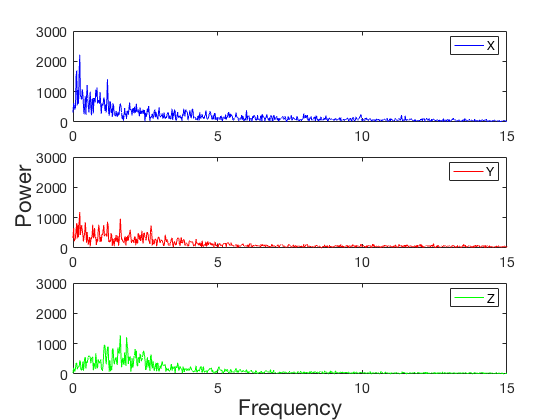
\includegraphics[width=.6\textwidth]{figures/gyroFFTPlot}
	\caption{The power spectral density of gyroscope data from the left leg of one subject.}
	\label{fig:gyroFFTPlot}  %<--remember LABEL!
\end{figure}



%MATLAB alignment GUI description
\subsection{Data Alignment}
Because the measurements from the FSRs are run on an Arduino, and the gyroscopes run through a Shimmer Sensing developed script for MATLAB, the timing for the measurements are run differently. In order to analyse FSR data to the corresponding time for gyroscope data a data alignment GUI have been developed in MATLAB. The implemented alignment program is a simple GUI which creates a plot where different channels from the six FSRs and six DoFs from the gyroscopes (three for each on each leg) can be shown or hidden. Additionally each channel can be translated left or right. This enables to align data from the FSRs to the gyroscopes, based on a spike in measurements caused by a small jump subjects will be asked to perform before and after performance of Pinan Nidan. An example of the alignment GUI in work can be seen in \figref{fig:alignGUI}.

\begin{figure}[H]
	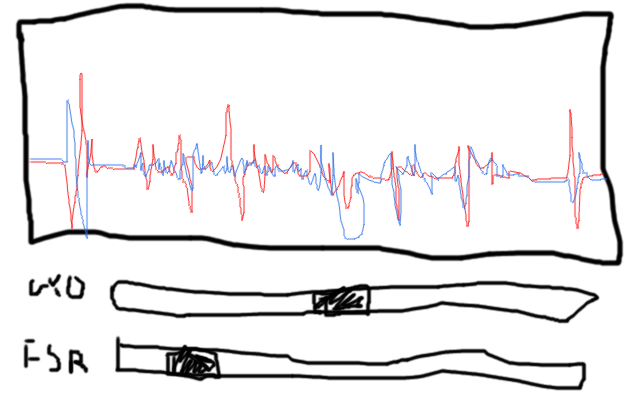
\includegraphics[width=.6\textwidth]{figures/alignGUI}
	\caption{The alignment GUI showing a selected number of channels from the FSRs and gyroscopes. All channels can be translated in order to align timestamps for the FSR measurements to timestamps for the gyroscopes.}
	\label{fig:alignGUI}  %<--remember LABEL!
\end{figure}


\subsection{Calculation of movement scores}

For calculating a movement score four separate scores will be calculated; COP, length, span and frequency distribution. COP is a calculation of the estimated COP for a test subject on a plane. The length is calculated on the path of the moving COP during recording. Span is a calculation of the area in which the COP has travelled. Frequency distribution is a measure for the gyroscope frequencies measured during recordings.

\subsubsection{Calculation of Centre of Pressure}
%method for calculation of COP 
%MATLAB COP code description
The COP (check for prior use of abbreviation) calculation consists of two simple equations to find the displacement of balance in the X and Y directions. To ensure the calculated values are unrelated to the weight of the test subject, but solely describes the displacement of balance, each calculation of the pressure distribution will be divided by the overall pressure placed on all sensors. The COP\lowercase{x} equation finds the distribution of weight between the two feet, whereas the COP\lowercase{y} equation describes the distribution between the sensors on the front and back of the foot. The COP measure is used in calculations of the length and span measures. In addition to the displacement of these sensors in relation to each other and to compensate for the number of sensors on the front and back of the foot, a weight ($W$) will be added to the pressure readings ($P$).
The COP calculations for X and Y directions follow \eqref{eq:COPx} and \eqref{eq:COPy}:

\begin{equation} \label{eq:COPx}
COP_x(i) =  \frac{\sum_{i=1}^{3}P_i W_i - \sum_{i=4}^{6}P_i W_i}{\sum_{i=1}^{6}P_i W_i}
\end{equation} 

\begin{equation} \label{eq:COPy}
COP_y(i) =  \frac{\sum(P_3 W_3 + P_6 W_6) - \sum(P_1 W_1+P_2 W_2+P_4 W_4+P_5 W_5)}{\sum_{i=1}^{6}P_i W_i}
\end{equation} 


%method for calculating scores based on calculated COP and gyroscope data

\subsubsection{Calculation of length score}
The length of the COP outcomes was calculated and divided by the length ($L$) of the recorded data, so the outcome measure described the mean COP change between each sample. To ensure this measure had an effect on the final score it was multiplied by a factor of 10. The length was calculated individually for X and Y directions for later use in score calculation (see \eqref{eq:length}).

\begin{equation} \label{eq:length}
	Length_{x,y} = \frac{\sum_{i=1}^{L-1}\sqrt{(COP_{x,y} (i+1)-COP_{x,y} (i))^2}}{L} * 10
\end{equation}


\subsubsection{Calculation of span score}
Calculation of the span describes the span between the outer most points of the COP changes, giving an area in which the COP travels. 
The span is calculated by taking the absolute value of the difference between maximum and minimum observed values of COP. This is calculated for both the X and Y directions. In the same manner as the length measure is scaled by a factor of 10, the span measure is divided by 10 to decrease the effect of the span in relation to the other measures. Span is calculated as shown in \eqref{eq:span}:
%Start out by finding min and max of scaled COP and difference between these values. Sum and abs of difference to find final span value. This is then divided by 10 for scaling in score calculation.

\begin{equation} \label{eq:span}
Span_{x,y} = \frac{\left| max(COP_{x,y})-min(COP_{x,y})\right|}{10}
\end{equation}


\subsubsection{Calculation of frequency distribution}
As described in \subref{subsec:filtering} on filtering, it is shown that the power spectrum of the gyroscope data provided very little information above 10Hz. Thus, the frequencies have been divided into two categories: low and high. Here, low frequencies is defined as 2/3 of the frequency spectrum from 0 to 5Hz, and are an expression for stable movements. High frequencies are defined as the last 1/3 of the frequency spectrum from 0 to 5Hz, and are an expression for less stable movements. This separation of low and high frequencies, relative to the frequency band of acquired data, is based on when the frequency distribution deviated less than 5\% of the mean for individual subject. The frequency distribution is calculated by the difference between the power at frequencies in the low and high category, divided by the total power of frequencies between 0 and 5Hz, as shown in \eqref{eq:fd}:

\begin{equation} \label{eq:fd}
Distribution = \frac{LowFreq-HighFreq}{LowFreq+HighFreq}
\end{equation}


\subsection{Calculation of performance score}
Each movement score; length, span and frequency distribution is used to calculate a final performance score for each subject. 
The performance score is calculated by dividing length by span, and multiplying by one subtracted with the frequency distribution, as seen in \eqref{eq:score}. The best performance score is produced by short lengths in relation to larger spans. The performance score is better the lower the value. 

%Having a short length for a movement sequence would mean precise path directly from start to finish, while a longer length would mean that a longer path have been taken between start and finish. A great span measure is a result of greater force excessed on the FSRs, meaning that movements have been performed faster. 
%lille lenght = præcis movement

\begin{equation} \label{eq:score}
Score = \frac{Length}{Span} * (1 - Frequency Distribution)
\end{equation}

%(10/10)*(1-0,5) = 0,5
%(10/1)*(1-0,5)   = 5
%(1/10)*(1-0,5)   = 0,05


